%!TEX root = ../main.tex
% =============================================================
% CAPÍTULO 4 — MARCO TECNOLÓGICO · MARKETLENS
% Adaptación del documento original y del esquema de la cátedra.
% Requiere los PNG 2 a 6 en figuras/marketlens/.
% Los datos de versiones no confirmadas se declaran expresamente.
% =============================================================

\chapter{Marco tecnológico}\label{cap:marco-tecnologico}

El presente capítulo describe las decisiones técnicas adoptadas para el desarrollo de MarketLens. Se distinguen los componentes que cuentan con evidencia de funcionamiento en el prototipo, las interfaces cuya integración es parcial y las capacidades incluidas en el diseño pero pendientes de implementación o validación. La arquitectura busca posibilitar el análisis preventivo de publicaciones sin depender exclusivamente de una interfaz de usuario ni del acceso irrestricto a datos de terceros.

\section{Arquitectura del sistema}\label{sec:ml-arquitectura}

\subsection{Estilo arquitectónico y justificación}\label{subsec:ml-estilo}

Se adoptó una \textbf{arquitectura cliente--servidor organizada en capas}. La presentación se distribuye entre una aplicación web y una extensión de navegador; ambos clientes se comunican con servicios HTTP del backend. En el servidor se separan las responsabilidades de controladores, servicios de negocio, evaluación de riesgo y acceso a datos. La persistencia se realiza en PostgreSQL.

Esta organización permite reutilizar la evaluación desde clientes diferentes y modificar las reglas del motor sin incorporar esas reglas en la interfaz. Además, el aislamiento de la obtención de datos facilita considerar diferentes fuentes de información y manejar sus restricciones. La figura~\ref{fig:ml-arquitectura-general} reproduce el esquema arquitectónico del documento original.

\begin{figure}[htbp]
    \centering
    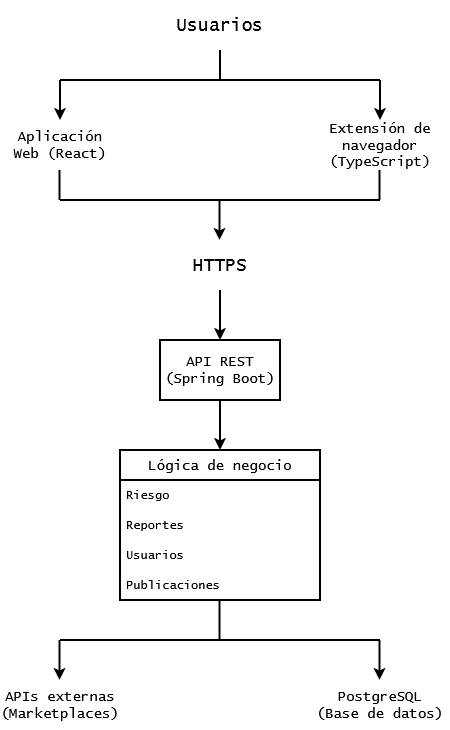
\includegraphics[width=0.66\textwidth,height=0.70\textheight,keepaspectratio]{figuras/marketlens/image2.png}
    \caption{Arquitectura general de MarketLens: clientes, API, lógica de negocio, fuentes externas y persistencia}
    \label{fig:ml-arquitectura-general}
\end{figure}

La selección privilegia la trazabilidad y el costo de mantenimiento de un prototipo académico. Una solución basada en microservicios independientes podría aislar procesos y escalar cada componente por separado, pero requeriría resolver descubrimiento de servicios, despliegues y comunicación distribuida sin que el volumen y la operación comprobados lo justifiquen. Por ello, se optó por un backend modular con responsabilidades diferenciadas, con la posibilidad de separar servicios en iteraciones futuras.

\begin{table}[htbp]
\centering
\caption{Decisiones arquitectónicas y alternativas consideradas}
\label{tab:ml-decisiones-arquitectura}
\small
\begin{tabularx}{\textwidth}{@{}p{0.22\textwidth} X X@{}}
\toprule
\textbf{Decisión adoptada} & \textbf{Justificación para el prototipo} & \textbf{Alternativa y motivo para no adoptarla inicialmente} \\
\midrule
Backend modular en capas & Separación de controladores, servicios, lógica de evaluación y persistencia; menor complejidad de operación & Microservicios: despliegue y coordinación distribuidos no justificados por el alcance comprobado \\
API REST compartida & Un mismo mecanismo de análisis puede atender al frontend y a la extensión & Lógica replicada en cada cliente: duplicación y diferencias de criterios \\
Persistencia relacional & Relaciones entre vendedor, publicaciones y evaluaciones; integridad de datos y consultas estructuradas & Almacenamiento exclusivamente documental: no aporta una ventaja clara a las relaciones centrales del prototipo \\
Extensión complementaria & Permite obtener datos visibles cuando las interfaces externas no ofrecen todos los atributos & Dependencia exclusiva de APIs de terceros: cobertura limitada por permisos y disponibilidad \\
\bottomrule
\end{tabularx}
\end{table}

\subsection{Responsabilidades de los componentes}\label{subsec:ml-componentes}

La \textbf{aplicación web}, desarrollada con React y TypeScript, permite autenticarse y acceder a las áreas de consulta de publicaciones, vendedores y dashboard. La información presentada procede de servicios del backend; el cliente no debe constituir una fuente autónoma de reglas de riesgo.

La \textbf{extensión de navegador} funciona como interfaz contextual mientras se consulta un marketplace. Durante las pruebas se utilizaron scripts de extensión y un popup para recopilar determinados atributos visibles y solicitar una evaluación. Su implementación probada utiliza archivos JavaScript; el uso de TypeScript aparece en el diseño como alternativa de evolución. Las APIs y permisos de extensiones condicionan qué acciones puede realizar este tipo de cliente \citep{ml-mdn-webextensions}.

El \textbf{backend}, implementado en Java con Spring Boot, centraliza los controladores REST, la gestión de publicaciones y vendedores, el procesamiento de evaluaciones y el acceso a persistencia. Spring Boot ofrece mecanismos de configuración y ejecución adecuados para aplicaciones web autónomas \citep{ml-spring-boot-docs}. El \textbf{motor de riesgo} se ubica en la capa de negocio: recibe atributos normalizados, evalúa reglas, produce la puntuación y registra factores explicativos. La \textbf{base de datos PostgreSQL} conserva los registros que pueden recuperarse desde los servicios.

Las \textbf{interfaces con marketplaces} actúan como fuentes complementarias y no como componentes controlados por MarketLens. La información que devuelven puede variar según los permisos, el recurso solicitado y la modalidad de publicación. La separación de responsabilidades se resume en la tabla~\ref{tab:ml-responsabilidades}.

\begin{table}[htbp]
\centering
\caption{Componentes y responsabilidades principales}
\label{tab:ml-responsabilidades}
\small
\begin{tabularx}{\textwidth}{@{}p{0.24\textwidth} X p{0.26\textwidth}@{}}
\toprule
\textbf{Componente} & \textbf{Responsabilidad} & \textbf{Estado documentado} \\
\midrule
Aplicación web & Autenticación, navegación y consulta de datos y estadísticas & Interfaz y comunicación inicial comprobadas \\
Extensión & Lectura de atributos visibles e inicio de análisis desde una publicación & Probada sobre determinadas páginas de Mercado Libre \\
API REST & Recepción de solicitudes, coordinación de servicios y respuestas JSON & Endpoints de publicaciones y evaluación utilizados en pruebas \\
Motor de riesgo & Reglas, ponderaciones, cobertura y comparación de precios & Casos funcionales y pruebas automatizadas registrados \\
PostgreSQL & Persistencia de publicaciones, vendedores y evaluaciones & Almacenamiento y recuperación comprobados \\
Reportes colaborativos & Recepción de contribuciones y su eventual revisión & Capacidad prevista; sin evidencia integral suficiente \\
\bottomrule
\end{tabularx}
\end{table}

\section{Flujos de información e integración}\label{sec:ml-flujos}

\subsection{Análisis de publicaciones}\label{subsec:ml-flujo-analisis}

El flujo de análisis comienza cuando un usuario consulta una publicación compatible, abre la extensión y solicita su evaluación. La información visible o previamente registrada se transmite a la API; el backend completa los atributos que están disponibles, ejecuta la lógica de negocio, registra los resultados pertinentes y devuelve una respuesta interpretable. La aplicación web puede consultar los datos almacenados sin reproducir el proceso de cálculo en el navegador.

La figura~\ref{fig:ml-interaccion-extension} representa la interacción inicial con la extensión. La figura~\ref{fig:ml-flujo-analisis} desarrolla el recorrido entre cliente, servicios, fuentes externas, motor de evaluación y persistencia. Ambos diagramas son \textbf{esquemas del proceso previsto}; las pruebas del capítulo~\ref{cap:resultados} acreditan únicamente los pasos documentados en los casos realizados.

\begin{figure}[htbp]
    \centering
    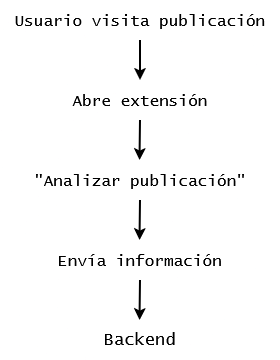
\includegraphics[width=0.47\textwidth,height=0.56\textheight,keepaspectratio]{figuras/marketlens/image3.png}
    \caption{Interacción del usuario con la extensión de navegador}
    \label{fig:ml-interaccion-extension}
\end{figure}

\begin{figure}[htbp]
    \centering
    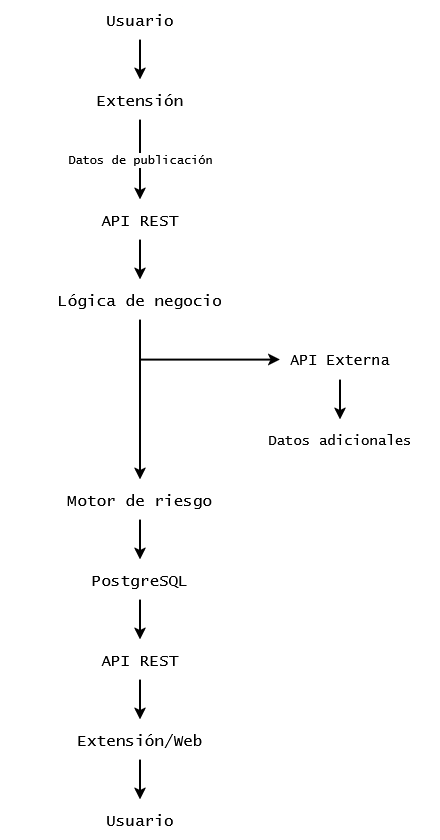
\includegraphics[width=0.64\textwidth,height=0.69\textheight,keepaspectratio]{figuras/marketlens/image5.png}
    \caption{Flujo general de análisis de una publicación y consulta de fuentes externas}
    \label{fig:ml-flujo-analisis}
\end{figure}

Entre las rutas utilizadas en las comprobaciones se encuentran \texttt{POST /api/publications}, para registrar una publicación; \texttt{GET /api/publications/70/price-analysis}, para inspeccionar su comparación de precios; y \texttt{POST /api/publications/70/evaluations}, para generar una evaluación. Los identificadores y rutas concretas son ejemplos del prototipo y no constituyen una especificación pública completa de la API. Las respuestas de prueba se documentan en el capítulo~\ref{cap:resultados} y el Apéndice A.

\subsection{Extracción de datos y límites de interoperabilidad}\label{subsec:ml-extraccion}

En las pruebas con Mercado Libre se emplearon dos fuentes posibles: servicios externos autorizados, cuando la consulta estaba disponible, y datos visibles de la página recuperados desde la extensión. Esta segunda vía permitió identificar información de vendedores y publicaciones en casos donde las respuestas de la API no aportaban todos los atributos requeridos. La integración no garantiza acceso uniforme a datos de terceros.

Se observaron diferencias de estructura entre publicaciones individuales y de catálogo; estas últimas todavía requieren ajustes adicionales. Por esa razón, el sistema distingue entre \textit{dato no disponible} y \textit{valor negativo comprobado}. En particular, no conocer el número de ventas o la antigüedad de una cuenta no equivale a registrar cero ventas o una cuenta recién creada. El tratamiento de ausencias también condiciona la cobertura informada en el resultado.

\subsection{Flujo de reportes colaborativos}\label{subsec:ml-flujo-reportes}

El diseño contempla que un usuario pueda registrar una observación sobre una publicación, adjuntar evidencia cuando corresponda y enviarla a un servicio que valide la entrada antes de almacenarla. Los registros podrían alimentar procesos de análisis y estadísticas agregadas. La figura~\ref{fig:ml-flujo-reportes} representa ese flujo conceptual.

\begin{figure}[htbp]
    \centering
    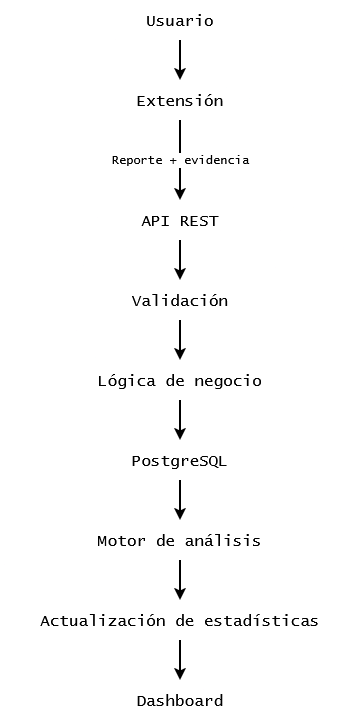
\includegraphics[width=0.61\textwidth,height=0.69\textheight,keepaspectratio]{figuras/marketlens/image6.png}
    \caption{Flujo previsto para la recepción y el tratamiento de reportes colaborativos}
    \label{fig:ml-flujo-reportes}
\end{figure}

El reporte de un usuario debe considerarse una fuente sujeta a corroboración, no una declaración concluyente de fraude. La evidencia registrada en la etapa actual no basta para afirmar que el circuito completo de reportes, moderación y análisis agregado haya sido validado con usuarios finales.

\section{Pila de software y criterios de elección}\label{sec:ml-stack}

El stack combina tecnologías para clientes web, servicios de negocio, persistencia, pruebas y control de versiones. La elección considera adecuación funcional, costos de adopción, experiencia adquirida durante el desarrollo y compatibilidad con una arquitectura modular. En la tabla~\ref{tab:ml-stack} se diferencian las tecnologías cuya utilización está documentada de aquellas previstas para un despliegue posterior. La \textbf{versión exacta} de cada dependencia debe contrastarse con los archivos \texttt{pom.xml}, \texttt{package.json}, el gestor de extensiones y la instalación de PostgreSQL antes de presentar una matriz definitiva de versiones.

\begin{table}[htbp]
\centering
\caption{Stack de MarketLens y estado de verificación de versiones}
\label{tab:ml-stack}
\small
\begin{tabularx}{\textwidth}{@{}p{0.18\textwidth}p{0.28\textwidth}X@{}}
\toprule
\textbf{Capa} & \textbf{Tecnología} & \textbf{Versión / justificación y alcance} \\
\midrule
Backend & Java, Spring Boot, Maven & Spring Boot 4.0.8 fue informado durante el desarrollo; verificar \texttt{pom.xml} actual. Servicios y pruebas en Java \\
Frontend & React, TypeScript, Vite & Versiones por verificar en \texttt{package.json}; interfaz de navegación y consultas \\
Extensión & JavaScript y APIs de extensión & Versión de manifiesto y navegador por verificar; scripts probados en la extensión \\
Persistencia & PostgreSQL & Versión instalada por verificar; relaciones entre registros y consultas estructuradas \\
Seguridad & Spring Security, JWT, BCrypt & Configuración documentada en el desarrollo; aplicación efectiva de controles sujeta a pruebas adicionales \\
Pruebas & JUnit, Maven y herramientas HTTP & Versiones por verificar; suite automatizada y comprobaciones funcionales \\
Entorno y código & Git, GitHub Desktop; Docker previsto & Git utilizado para versiones; contenerización y operación cloud no acreditadas integralmente \\
\bottomrule
\end{tabularx}
\end{table}

Para la capa de servicios se prefirió Spring Boot frente a una solución Java de configuración manual por la integración entre controladores, seguridad, acceso a datos y gestión de dependencias; se evitó introducir una pila nueva sin una necesidad demostrada. En la interfaz, React y TypeScript permiten organizar componentes y mantener contratos de datos explícitos. Para persistencia se eligió un sistema relacional en lugar de una base exclusivamente documental, ya que la estructura de publicaciones, vendedores y evaluaciones requiere relaciones consistentes. PostgreSQL permite expresar claves y restricciones referenciales de forma declarativa \citep{ml-postgresql-constraints}.

La comparación de productos se implementó mediante normalización, TF--IDF y similitud coseno, sin depender de un modelo predictivo entrenado para clasificar fraude. Esta decisión permite inspeccionar y ensayar reglas sobre un conjunto limitado de ejemplos, aunque no resuelve por sí sola los problemas de equivalencia comercial o validación estadística. Sus fundamentos se presentan en el capítulo~\ref{cap:marco-teorico}, particularmente a partir de \citet{ml-manning-2008}.

\section{Persistencia y modelo de datos}\label{sec:ml-persistencia}

La capa de datos del prototipo se apoya en PostgreSQL. Las entidades utilizadas en las pruebas incluyen \textbf{vendedor}, \textbf{publicación} y \textbf{evaluación de riesgo}. Cada publicación se vincula con la información disponible de un vendedor y puede conservar más de una evaluación para documentar revisiones de las reglas o del registro analizado. La tabla~\ref{tab:ml-entidades} describe el modelo lógico central; no sustituye un diagrama entidad--relación ni una inspección de los esquemas SQL definitivos.

\begin{table}[htbp]
\centering
\caption{Entidades centrales y relaciones lógicas del prototipo}
\label{tab:ml-entidades}
\small
\begin{tabularx}{\textwidth}{@{}p{0.24\textwidth} X X@{}}
\toprule
\textbf{Entidad} & \textbf{Datos y función} & \textbf{Relación principal} \\
\midrule
Vendedor & Identificador y atributos observables de trayectoria y reputación, con información temporal cuando está disponible & Un vendedor puede aparecer asociado a varias publicaciones \\
Publicación & Identificador, título, precio, estado y otros datos registrados para su análisis & Referencia a vendedor; base de evaluaciones \\
Evaluación de riesgo & Puntuación, nivel, factores, cobertura y momento de evaluación & Varias evaluaciones pueden corresponder a una publicación \\
\bottomrule
\end{tabularx}
\end{table}

El diseño más amplio también contempla usuarios, reportes, marketplaces e historial de actividad; su presencia en el modelo conceptual no implica que todas esas relaciones hayan sido verificadas con pruebas de persistencia. Para la evolución del esquema se recomienda documentar claves foráneas, índices, restricciones de integridad y procedimientos de migración según las consultas reales del sistema.

\section{Motor de evaluación de riesgo}\label{sec:ml-motor}

\subsection{Procesamiento y cobertura de información}\label{subsec:ml-procesamiento-riesgo}

El motor recibe los atributos recopilados de una publicación y su vendedor, identifica qué datos son utilizables y aplica las reglas pertinentes. La figura~\ref{fig:ml-flujo-motor} representa el proceso conceptual desde la extracción de características hasta el almacenamiento del resultado.

\begin{figure}[htbp]
    \centering
    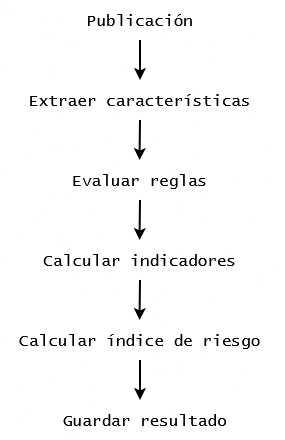
\includegraphics[width=0.54\textwidth,height=0.64\textheight,keepaspectratio]{figuras/marketlens/image4.png}
    \caption{Secuencia de procesamiento y evaluación prevista para el motor de riesgo}
    \label{fig:ml-flujo-motor}
\end{figure}

Se requiere distinguir tres situaciones: un atributo observado y evaluable, un atributo ausente y un atributo presente pero cuya interpretación resulta insuficiente. La falta de datos no debe traducirse automáticamente en penalización. Por ello, el sistema comunica una \textbf{cobertura} asociada a la disponibilidad de factores. En la evaluación de la publicación interna \#70 se registró cobertura parcial de dos factores evaluables sobre tres considerados; el índice obtenido fue de 40/100, pero no equivale a una probabilidad de fraude del 40\,\%.

\subsection{Comparación automática de precios}\label{subsec:ml-comparador-precios}

Para identificar candidatos potencialmente comparables se normalizan los títulos y se utiliza su representación TF--IDF, junto con la similitud coseno. La evaluación incorpora verificaciones complementarias para detectar discrepancias relevantes de modelo, capacidad, condición o composición de un paquete. La similitud textual, por sí sola, no constituye prueba de equivalencia comercial.

Cuando existen referencias suficientemente justificadas, se calculan medidas descriptivas como mediana, cuartiles, rango intercuartílico y diferencia relativa de precio. La ecuación~\ref{eq:ml-diferencia-precio}, presentada en el capítulo metodológico, define la desviación relativa respecto de la referencia utilizada. Si el número o la calidad de las referencias no permite sustentar una inferencia, el motor evita aplicar una penalización adicional por precio basada en estadísticas insuficientes.

La implementación mostró ambos comportamientos: un caso con una sola referencia provisional no generó penalización por precio, mientras que la publicación \#70 obtuvo 12 referencias automáticas, una mediana de ARS~1.499.950 y una diferencia de aproximadamente $-50{,}60$\,\% respecto de su precio. La equivalencia comercial de todas esas ofertas no quedó confirmada; el propio servicio informó el carácter experimental de su percentil. Los resultados y sus límites se desarrollan en el capítulo~\ref{cap:resultados}.

\subsection{Puntuación y explicación del resultado}\label{subsec:ml-interpretacion-riesgo}

La evaluación se expresa mediante un puntaje entre 0 y 100, una categoría cualitativa y las contribuciones de los factores utilizados. Durante el proceso de desarrollo se revisaron ponderaciones en un caso de prueba: el factor por precio anormalmente bajo pasó de 15 a 25 puntos, y el factor por historial comercial limitado pasó de 10 a 15 puntos. La evaluación posterior registró un total de 40 puntos y nivel \texttt{MEDIUM}. Este cambio se documenta como una modificación deliberada de reglas y no como evidencia de mejora de la precisión frente a fraudes reales.

El índice representa un resultado de reglas de negocio, no una clasificación validada mediante un conjunto etiquetado de operaciones fraudulentas. La interpretación requiere presentar los factores considerados, la cobertura y las limitaciones de datos junto con la puntuación.

\section{Diseño de interfaz y experiencia de usuario}\label{sec:ml-ux}

El diseño contempla dos situaciones de uso: la consulta desde una aplicación web centralizada y la evaluación contextual desde un marketplace mediante la extensión. En el frontend se organizaron áreas de dashboard, vendedores y publicaciones, y se incorporó una interfaz de autenticación. El popup de la extensión busca presentar de forma compacta la puntuación, el nivel de riesgo, la cobertura y las razones de la evaluación. La figura~\ref{fig:ml-extension-70}, en el capítulo~\ref{cap:resultados}, muestra una captura correspondiente a la publicación \#70.

La separación visual entre \textbf{puntuación}, \textbf{nivel} y \textbf{cobertura} responde a una necesidad de interpretación: un puntaje por sí solo puede sugerir certeza excesiva cuando faltan datos. Las decisiones visuales incluyeron contrastes de tarjetas y alternativas de tema claro y oscuro durante el desarrollo. Sin embargo, no se cuenta en el informe con una evaluación formal de usabilidad mediante una muestra de usuarios o expertos. Por tanto, no se atribuyen al diseño mejoras medidas de comprensión, accesibilidad o satisfacción; esas comprobaciones se proponen como trabajo futuro.

\section{Seguridad, pruebas y despliegue}\label{sec:ml-seguridad-calidad}

\subsection{Protección de servicios y datos}\label{subsec:ml-seguridad}

El backend incorporó mecanismos de autenticación y autorización mediante Spring Security, con emisión y validación de tokens JWT y uso de BCrypt para proteger contraseñas. En el desarrollo se empleó un esquema de firma JWT con clave secreta configurada externamente; su protección y rotación son condiciones relevantes para un eventual despliegue productivo. Estas medidas no sustituyen las pruebas de seguridad sobre rutas, permisos y exposición de información.

Las comprobaciones locales se realizaron mediante servicios HTTP en \texttt{localhost}. Para un despliegue público se requiere proteger las comunicaciones mediante HTTPS, restringir la conexión directa a la base de datos, administrar credenciales fuera del código fuente, validar entradas y registrar errores sin exponer información sensible. La presencia de controles en el diseño no equivale a una auditoría de seguridad terminada.

\subsection{Verificación funcional y automatizada}\label{subsec:ml-pruebas-calidad}

La estrategia de verificación comprende pruebas automatizadas de reglas y servicios, comprobaciones HTTP y pruebas de integración con la extensión. Los casos de referencia analizan la ausencia de penalización ante evidencia insuficiente, la acumulación de ponderaciones y la consistencia del resultado presentado por el cliente. En una ejecución registrada se informaron \textbf{62 pruebas automatizadas exitosas, sin fallos ni errores}. Ese resultado respalda el comportamiento de los escenarios ensayados, pero no demuestra la eficacia de MarketLens para reconocer estafas reales.

La trazabilidad entre indicadores operativos y pruebas se establece en la tabla~\ref{tab:ml-indicadores} del capítulo~\ref{cap:metodologia}, mientras que las evidencias funcionales se presentan en el capítulo~\ref{cap:resultados} y en los apéndices técnicos.

\subsection{Infraestructura, entrega y evolución}\label{subsec:ml-despliegue}

La etapa documentada utiliza una ejecución local del backend, de la base de datos y de los clientes de prueba. Git permite mantener versiones del código y de la documentación; el repositorio académico en GitHub constituye el mecanismo de entrega. Los contenedores y el alojamiento en servicios cloud forman parte de las alternativas de infraestructura previstas, pero no se declara una operación productiva continua, un sistema completo de integración y despliegue continuos ni monitoreo de producción que no hayan sido acreditados.

La estimación de costos de desarrollo, infraestructura y operación se presenta en el capítulo~\ref{cap:economica}. La selección definitiva de un proveedor de alojamiento debería considerar confidencialidad de datos, respaldo, disponibilidad, costo y compatibilidad con las restricciones de las fuentes externas.

\section{Alcance del prototipo y limitaciones técnicas}\label{sec:ml-limitaciones-tecnicas}

La implementación verificable demuestra la comunicación básica entre cliente, backend y persistencia, la obtención de algunos atributos visibles mediante la extensión y la ejecución del motor en escenarios definidos. Persiste una compatibilidad parcial con los distintos formatos de publicaciones de Mercado Libre y no se dispone de evidencia equivalente para otros marketplaces. Tampoco se ha establecido la completitud del circuito colaborativo de reportes ni su resistencia a contribuciones maliciosas.

En futuras iteraciones corresponderá ampliar la compatibilidad de extracción, validar mejor la equivalencia comercial entre referencias, formalizar pruebas de seguridad y accesibilidad, documentar el esquema SQL y medir el desempeño bajo carga. También será necesario contar con información de referencia externa para evaluar la calidad real de los indicadores de riesgo. La arquitectura modular adoptada permite abordar estas tareas sin confundir su posibilidad técnica con funcionalidades ya verificadas.

% =============================================================
% NOTAS EDITORIALES (NO SE IMPRIMEN)
% - Verificar versiones: pom.xml, package.json, motor PostgreSQL,
%   manifest.json de extensión antes de congelar la entrega final.
% - Integrar 3 entradas .bib provistas con este capítulo.
% - Se usan los archivos image2.png a image6.png ya extraídos de Word.
% - La referencia fig:ml-extension-70 requiere el capítulo 07 adaptado.
% - No atribuir al prototipo pruebas con usuarios ni despliegue cloud.
% - El modelo de datos presentado es lógico, no el DDL definitivo.
% =============================================================
